
%(BEGIN_QUESTION)
% Copyright 2008, Tony R. Kuphaldt, released under the Creative Commons Attribution License (v 1.0)
% This means you may do almost anything with this work of mine, so long as you give me proper credit

Below is an illustration of a diaphragm-operated {\it pressure switch}, designed to actuate when the process fluid pressure applied to the impulse line (tube) exceeds a certain set value.  A schematic diagram shows how the switch contacts relate to the screw terminals seen on the outside of the switch illustration:

$$\includegraphics[width=15.5cm]{i00222x01.eps}$$

Explain what is meant by the ``normally-closed'' (NC) and ``normally-open'' (NO) labels next to two of the electrical screw terminals.  Identify the status of the switch when process pressure exceeds the switch's set value.

\underbar{file i00222}
%(END_QUESTION)





%(BEGIN_ANSWER)

As with all process switches, the ``normal'' status refers to the electrical status of the switch in a condition of {\it minimum stimulus}.  In this particular case, when the process pressure is below the set value, the switch will be in its ``normal'' status (as drawn in the schematic), with electrical continuity between Com and NC, and no electrical continuity between Com and NO.

\vskip 10pt

It is very important to distinguish the ``normal'' status of a process switch from its ``typical'' status while installed in a working process.  For instance, if this switch's set value was 50 PSI, we could use it as a low pressure alarm (PAL) switch, whose duty it is to energize an alarm if the process pressure ever drops {\it below} 50 PSI.  In this case, the alarm circuit would use the Com and NC contacts on the switch, with regular process pressure (above 50 PSI) holding the normally-closed contact in its {\it open} state, letting that contact fall back to its ``normal'' (closed) state if the process pressure ever drops below 50 PSI.  Here, the NC contact {\it typically} resides in the open state, even though it is a ``normally closed'' contact, simply because of how we are using it in the process.

Some students may balk at this convention.  ``Why not call the contact either `normally-open' or `normally-closed' depending on which state that contact {\it normally} resides while operating in the process?'' they may ask.  The answer is simple: the switch manufacturer has no idea how you intend to use it.  How would they know whether to call the contact NO or NC, if they don't know the ``normal'' operating conditions of your process and the purpose for which you will use their switch?  The standard convention of defining ``normal'' switch contact status as that state in a condition of minimum stimulus (low pressure for a pressure switch, low temperature for a temperature switch, etc.), while potentially confusing, is actually less confusing than the alternative most students immediately envision.

%(END_ANSWER)





%(BEGIN_NOTES)


%INDEX% Switch, pressure: ``normal'' status of contacts

%(END_NOTES)


